% Fudan University graduate thesis template.
% Save this file as UTF-8 and compile it with XeLaTeX or LuaLaTeX.
% The supplied declaration is PDF 1.7; emit a matching version.
\PassOptionsToPackage{pdfversion=1.7}{hyperref}
\documentclass[type=doctor,twoside]{fduthesis}
% Change type=doctor to type=master when preparing a master's thesis.

\fdusetup{
  style = {
    font = times*,
    cjk-font = windows,
    font-size = -4,
    footnote-style = xits,
    hyperlink = none,
    logo = {assets/spec-cover-logo.png},
    bib-backend = bibtex,
    bib-style = numerical,
    bib-resource = {references.bib},
    % The class appends this PDF from its end-document hook. It is therefore
    % always the final page of the compiled thesis PDF.
    declaration-page = {assets/declaration.pdf},
    auto-make-cover = true,
  },
  info = {
    title = {中文论文题目},
    title* = {英文论文题目},
    author = {学生姓名},
    supervisor = {导师姓名 \quad 职称},
    major = {专业名称},
    degree = professional,
    department = {培养单位名称},
    student-id = {学号},
    date = {年\quad 月\quad 日}, % Replace with the actual submission date.
    instructors = {
      {导师姓名 \quad 职称},
    },
    keywords = {关键词一, 关键词二, 关键词三},
    keywords* = {keyword one, keyword two, keyword three},
    clc = {}, % Fill in the CLC classification code.
    applicant-type = {}, % 同等学力人员 or 英文项目, only when applicable.
  }
}

\usepackage{array}
\usepackage{booktabs}
\usepackage{longtable}
\usepackage{makecell}
\usepackage{tabularx}
\usepackage{threeparttable}
\usepackage{subcaption}
\usepackage{algorithm}
\usepackage{algpseudocode}
\usepackage{enumitem}
\usepackage{template-layout}
\usepackage{template-cover}

% Images in figures/ can be referenced without the directory or extension.
\graphicspath{{figures/}}
\DeclareGraphicsExtensions{.pdf,.png,.jpg,.jpeg}
\newcolumntype{Y}{>{\raggedright\arraybackslash}X}
\floatname{algorithm}{算法}
\algrenewcommand\algorithmicrequire{\textbf{输入：}}
\algrenewcommand\algorithmicensure{\textbf{输出：}}
\algrenewcommand\algorithmicreturn{\textbf{返回}}
% Template convention: number headings through \subsubsection.
\setcounter{secnumdepth}{3}

\begin{document}

\frontmatter

\tableofcontents
\begin{abstract}
中文摘要应独立说明研究背景、研究问题、方法、主要结果和结论。删除本段并替换为实际摘要；通常不在摘要中插图、列表、公式编号或参考文献。
\end{abstract}

\begin{abstract*}
Write the English abstract here. It should summarize the research background,
problem, method, main results, and conclusions without relying on the main
text. Replace this paragraph before submission.
\end{abstract*}

\listoffigures
\listoftables
% Delete the \input line for this file in main.tex when a notation list is not
% required. The notation environment automatically creates the front-matter
% heading and accepts the same column specification as a LaTeX table.
\begin{notation}[lp{8.2cm}]
  $a$ & 示例参数；请用一句话说明符号的物理、统计或工程含义。 \\
  $x_i$ & 第 $i$ 个观测值或输入变量。 \\
  $\mathbf{x}$ & 向量或矩阵变量；粗体与斜体的含义应在全文保持一致。 \\
  $\mathbb{E}[\cdot]$ & 数学期望算子。 \\
  $\mathrm{RMSE}$ & 均方根误差（root mean square error）。 \\
\end{notation}


\mainmatter

\chapter{绪论}
\label{chap:introduction}

\section{研究背景}

在这里介绍课题背景、研究价值和实际需求。首次出现的缩略语应给出中文名称、英文名称和缩写；后文保持同一术语与符号写法。需要补充而不宜放入正文的说明，可使用脚注。\footnote{这是脚注示例，使用带圈编号。学校规范建议采用脚注，但未统一规定编号样式。}

\section{研究现状}

按主题归纳已有工作，并在正文中使用 \verb|\cite{...}| 引用文献。例如，\cite{lamport1994latex,knuth1984literate} 分别给出了文档排版与可复现技术写作的经典讨论。不要把参考文献仅堆在段末，应说明它与当前论述的关系。

会议论文和网络资料的著录示例分别见文献\cite{vaswani2017attention,latexproject}。此处只演示不同文献类型的引用格式，实际写作时应替换为与研究内容相关的来源。

\section{本文工作与结构}

说明本文解决的问题、采用的技术路线和各章安排。可以用列表概括研究工作：

\begin{enumerate}[label=(\arabic*)]
  \item 明确研究对象、问题边界和评价指标；
  \item 说明方法、数据或实验设计；
  \item 给出结果、讨论局限性并形成结论。
\end{enumerate}

本模板在第~\ref{chap:method} 章给出公式、单图和定理的写法，在第~\ref{chap:results} 章给出三线表、表注、宽表、子图与算法的写法。删除不适用于本人的示例，不要在最终稿保留占位文字。

\chapter{方法与研究设计}
\label{chap:method}

\section{方法概述}

在本章说明研究对象、数据来源、实验条件或理论推导过程。图、表和公式应在正文中先被引用，再出现于相邻位置。图~\ref{fig:single-plot} 使用了模板自带的 PNG 示例文件，实际写作时请用自己的图片替换它。

\begin{equation}
  y_i = \alpha x_i + \beta + \varepsilon_i,
  \label{eq:linear-model}
\end{equation}

式~\eqref{eq:linear-model} 是公式编号与交叉引用的示例。行内公式写作 $y=f(x)$；只对需要单独讨论或在后文引用的公式使用 \texttt{equation} 环境。

彼此关联的多行推导可使用 \texttt{align} 环境，并只给需要引用的行添加标签：

\begin{align}
  \hat{y}_i &= \alpha x_i + \beta, \label{eq:prediction} \\
  \mathcal{L} &= \sum_{i=1}^{n}\left(y_i-\hat{y}_i\right)^2.
  \label{eq:loss}
\end{align}

式~\eqref{eq:prediction} 和式~\eqref{eq:loss} 分别给出预测值与示例损失函数。

\begin{figure}[htbp]
  \centering
  % Omit the extension so the same source can be supplied as PDF, PNG, or JPG.
  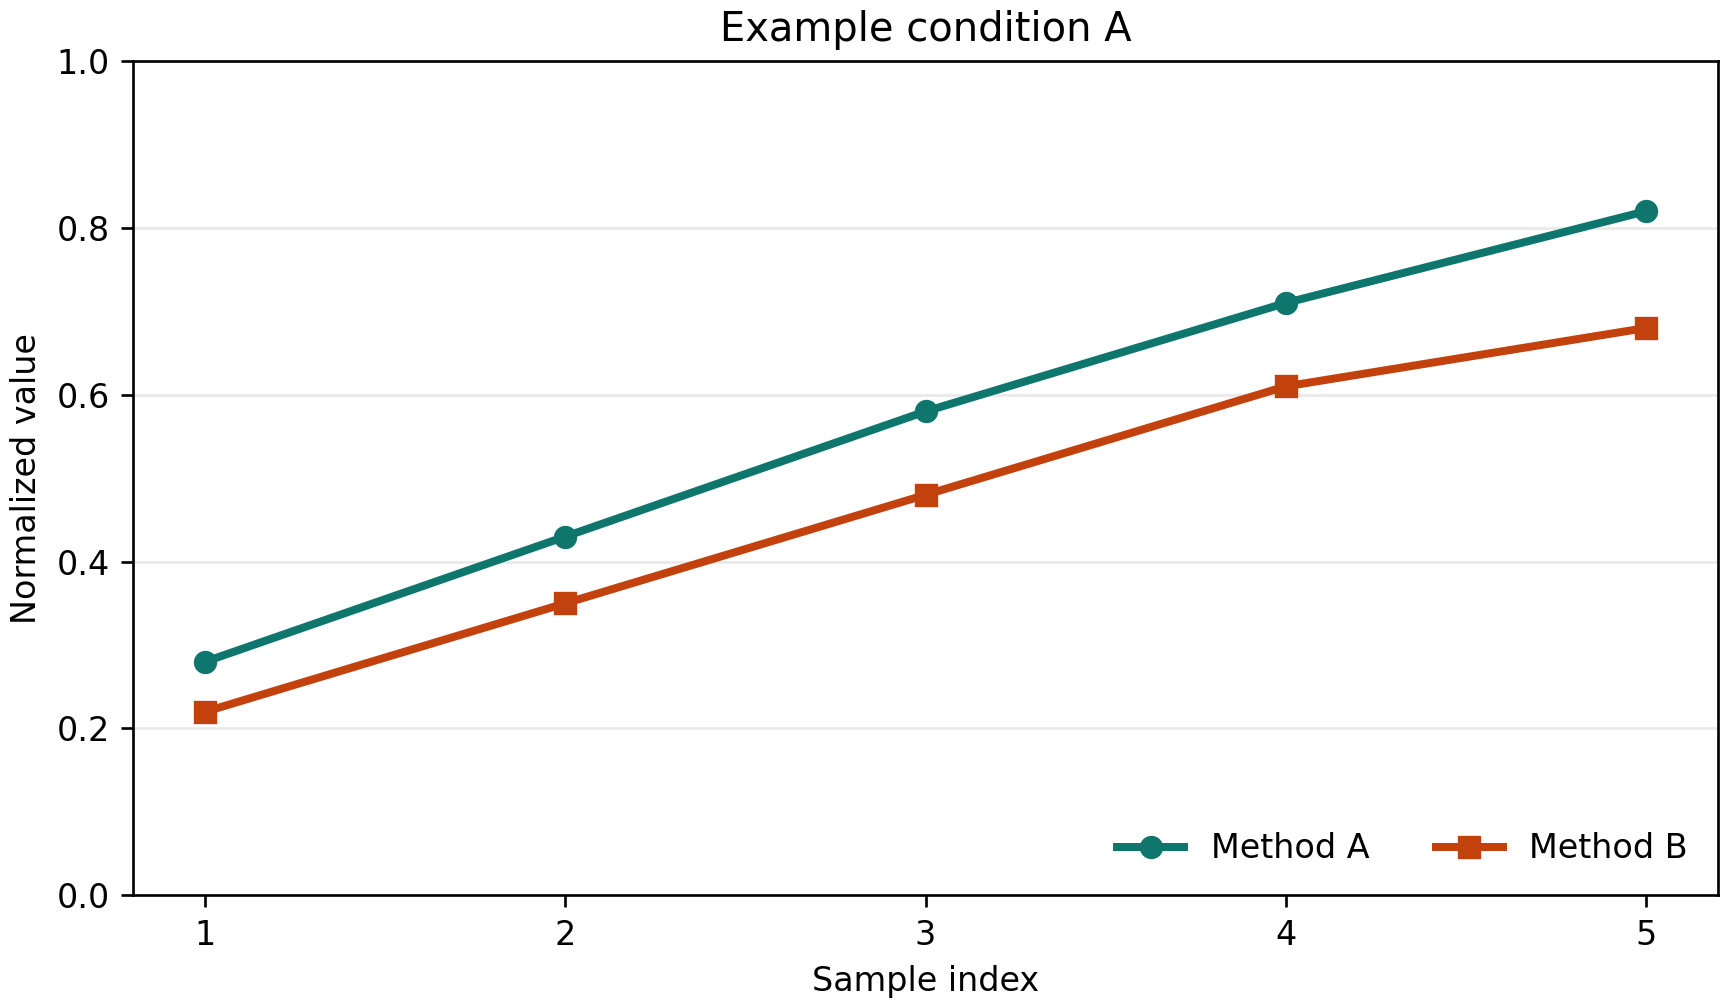
\includegraphics[width=0.74\textwidth]{example-plot-a}
  % 方括号内为插图清单中的独立名称，花括号内为正文图题。
  \caption[示例单图]{示例单图：请用自己的图片和说明替换}
  \label{fig:single-plot}
\end{figure}

\section{概念、定理与证明}

需要正式定义、定理或证明时，可直接使用类文件已提供的环境。

\begin{definition}[示例定义]
设 $\mathcal{D}$ 是研究对象的样本集合。若一个指标可以由 $\mathcal{D}$ 唯一计算，则称该指标在本研究设定下是可观测的。
\end{definition}

\begin{theorem}[示例命题]
若 $\varepsilon_i=0$ 且 $\alpha\ne0$，则式~\eqref{eq:linear-model} 中的 $x_i$ 可由 $y_i$ 唯一确定。
\label{thm:invertible-example}
\end{theorem}

\begin{proof}
由式~\eqref{eq:linear-model} 可得 $x_i=(y_i-\beta)/\alpha$。由于 $\alpha\ne0$，该表达式唯一，命题成立。
\end{proof}

定理~\ref{thm:invertible-example} 仅展示排版方式；最终论文应保留与研究内容有关且经过完整论证的定义和定理。

\begin{table}[htbp]
  \centering
  \caption{示例结果表}
  \label{tab:example}
  \begin{tabular}{lcc}
    \toprule
    方法 & 指标一 & 指标二 \\
    \midrule
    方法 A & 0.00 & 0.00 \\
    方法 B & 0.00 & 0.00 \\
    \bottomrule
  \end{tabular}
\end{table}

表~\ref{tab:example} 展示了三线表示例。需要插图时，将图像放在 \texttt{figures/} 目录，并使用 \verb|\includegraphics| 插入。

\chapter{结果与讨论}
\label{chap:results}

\section{表格与结果呈现}

表~\ref{tab:main-results} 展示了三线表、表注和交叉引用方式。标题在表格上方，标签命令应紧跟表题命令。表内小字号、加粗表头和无编号表注是本示例的排版选择，学校规范未统一规定。

\begin{table}[htbp]
  \centering
  \small
  \caption{示例结果汇总}
  \label{tab:main-results}
    \begin{tabular}{lcc}
      \toprule
      \textbf{方法} & \textbf{指标一} & \textbf{指标二} \\
      \midrule
      基线方法 & 0.72 & 12.4 \\
      提出方法 & 0.85 & 9.1 \\
      \bottomrule
    \end{tabular}
  \thesistablenote{数据仅用于演示三线表结构，请替换为实际实验结果。表注可解释缩写、统计检验、单位或数据来源。}
\end{table}

表~\ref{tab:wide-table} 演示 \texttt{tabularx} 的宽表写法。长文字放入 \texttt{Y} 列，避免通过缩小字号或压缩列间距强行塞入内容。

\begin{table}[htbp]
  \centering
  \small
  \caption{示例宽表}
  \label{tab:wide-table}
  \begin{tabularx}{\textwidth}{lYY}
    \toprule
    \textbf{项目} & \textbf{说明} & \textbf{报告建议} \\
    \midrule
    数据集 & 说明数据来源、时间范围、样本量与筛选规则。 & 报告训练、验证和测试集的划分方式。 \\
    实验设置 & 说明硬件、软件版本、关键参数及随机种子。 & 保证他人能够复现主要结果。 \\
    评价指标 & 给出指标定义、单位、方向和统计方法。 & 同时报告均值、波动或置信区间。 \\
    \bottomrule
  \end{tabularx}
\end{table}

\section{子图与算法}

当多个面板共同回答一个问题时，使用图~\ref{fig:subfigures} 这样的子图。若各图相互独立，应拆成多张图，不要为节省页数强行拼接。

\begin{figure}[htbp]
  \centering
  \begin{subfigure}[b]{0.48\textwidth}
    \centering
    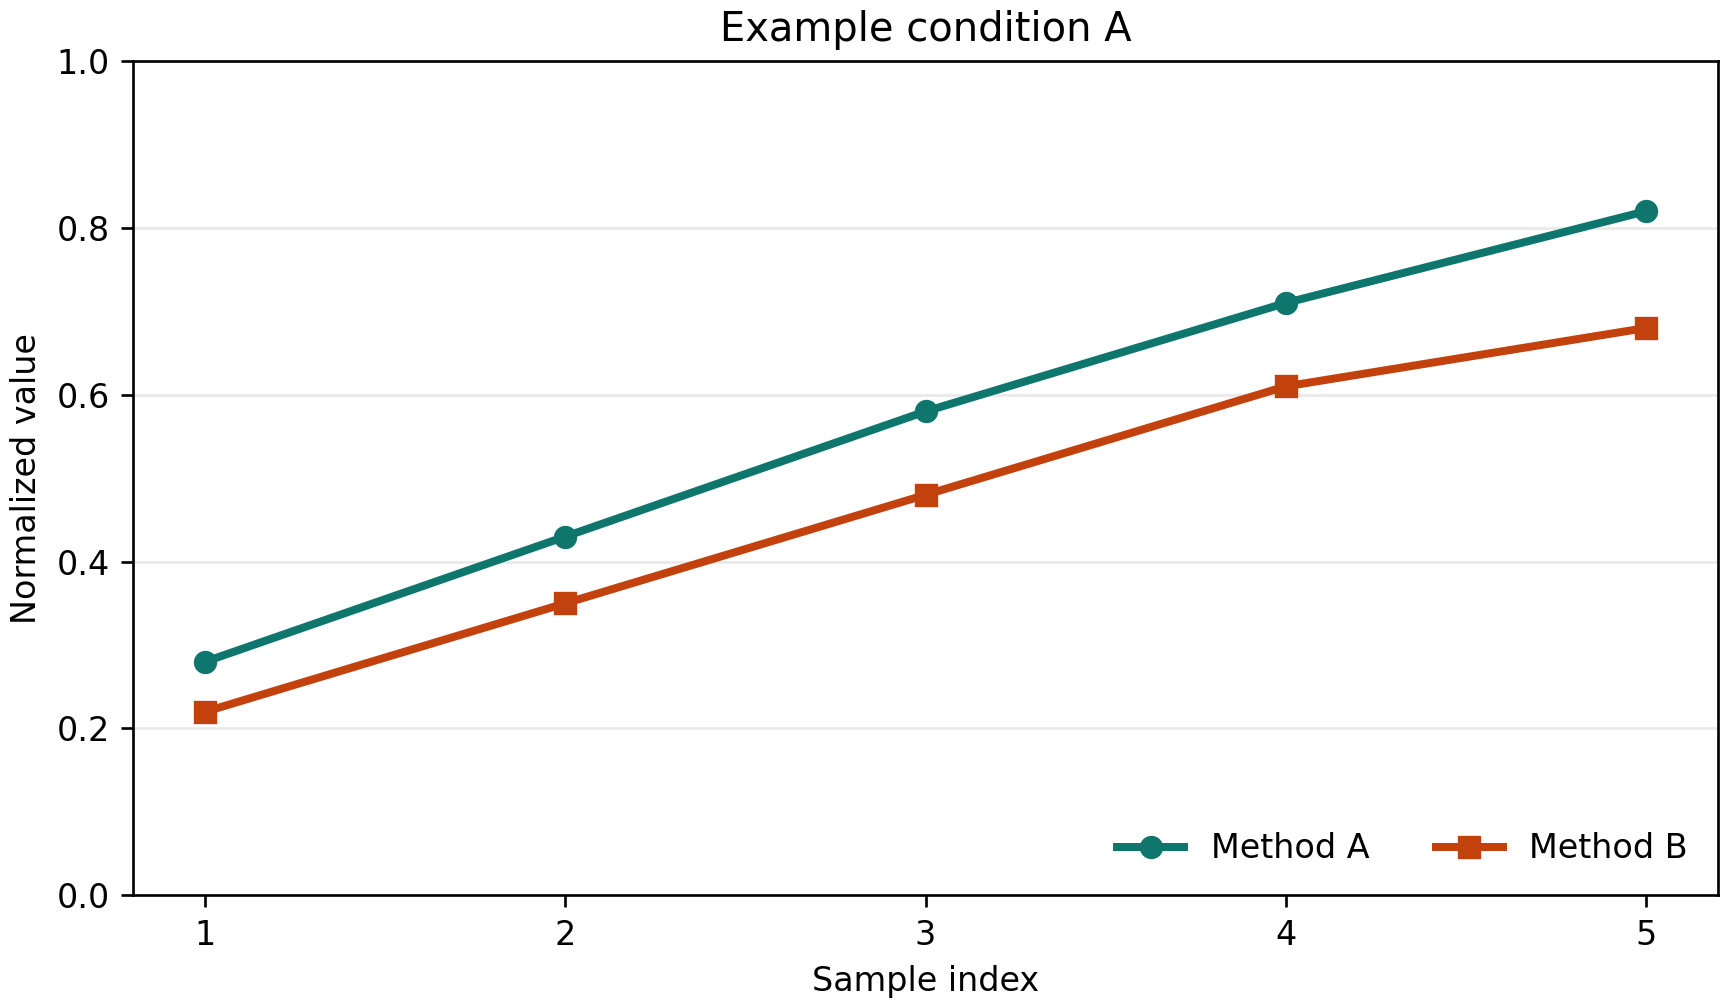
\includegraphics[width=\linewidth]{example-plot-a}
    \caption{}
    \label{fig:condition-a}
  \end{subfigure}
  \hfill
  \begin{subfigure}[b]{0.48\textwidth}
    \centering
    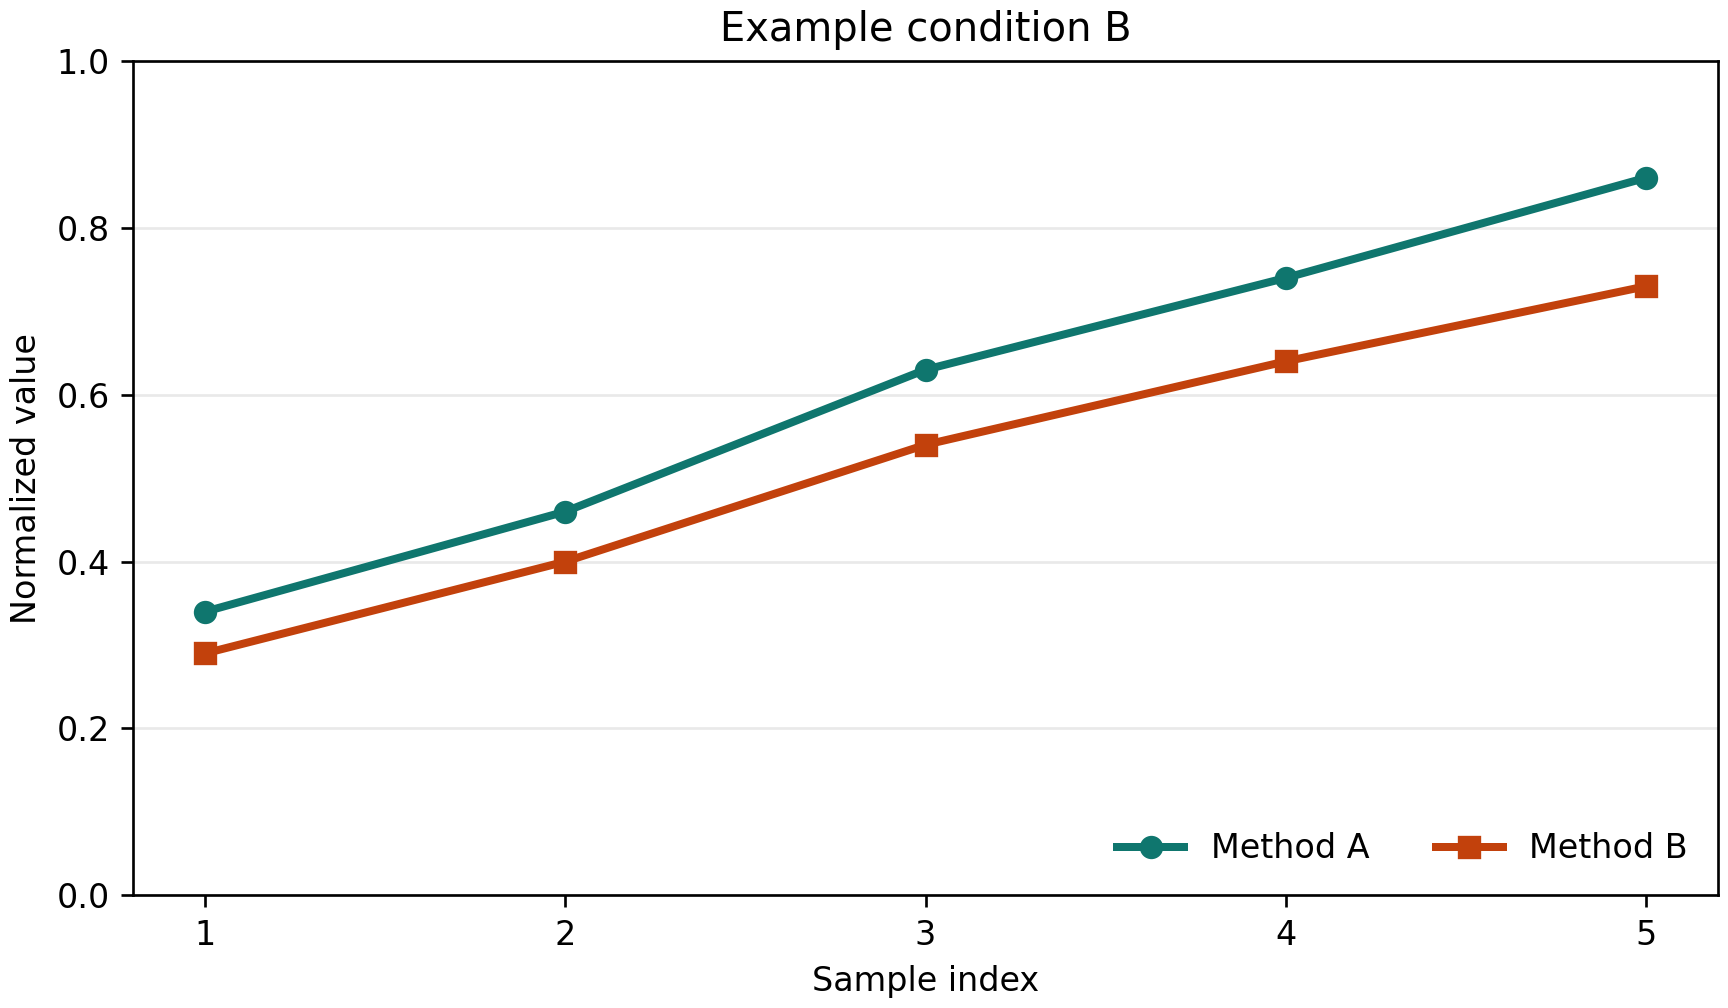
\includegraphics[width=\linewidth]{example-plot-b}
    \caption{}
    \label{fig:condition-b}
  \end{subfigure}
  % 组合图的插图清单名称写在总图题的方括号中。
  \caption[两种条件比较]{同一研究问题下的两种条件比较：（a）示例条件 A；（b）示例条件 B}
  \label{fig:subfigures}
\end{figure}

算法~\ref{alg:example} 演示伪代码环境。不要用截图展示算法；每一步应能与正文的输入、输出和符号对应。

\begin{algorithm}[htbp]
  \caption{示例处理流程}
  \label{alg:example}
  \begin{algorithmic}[1]
    \Require 输入数据集合 $\mathcal{D}$，阈值 $\tau$
    \Ensure 处理后的结果集合 $\mathcal{R}$
    \State 初始化 $\mathcal{R}\gets\varnothing$
    \For{每个样本 $d\in\mathcal{D}$}
      \State 计算评分 $s\gets f(d)$
      \If{$s\geq\tau$}
        \State 将 $d$ 加入 $\mathcal{R}$
      \EndIf
    \EndFor
    \State \Return $\mathcal{R}$
  \end{algorithmic}
\end{algorithm}

\chapter{结论与展望}
\label{chap:conclusion}

\section{主要结论}

概括本文解决的问题、得到的可验证结论和支持结论的证据。不要只重复各章标题，也不要在结论中提出尚未在正文论证的新结果。

\section{研究局限与展望}

说明研究的适用条件、数据或实验限制，以及值得继续开展的问题。对局限性的说明应具体，并与第~\ref{chap:results} 章的结果讨论相呼应。


\appendix
\chapter{补充材料示例}
\label{app:supplement}

将不适合放在正文、但有助于复现或理解论文的推导细节、问卷、补充实验、代码说明或数据字段定义放入附录。每个附录应能在正文中被引用，例如“见附录~\ref{app:supplement}”。

% Delete the next line if the college does not require an achievements section.
\chapter{攻读学位期间研究成果}

按学院当年要求列出与学位论文相关的学术论文、专利、项目或其他成果。删除不适用的小节，不保留空白占位项；成果的作者顺序、状态和编号应与正式记录一致。


\backmatter

\printbibliography
\begin{acknowledgements}
在此致谢对论文工作提供指导、协助或支持的个人和单位。致谢应真实、克制并符合学院要求；提交前删除本段占位文字。

此处可继续填写第二段致谢。各段之间空一行，首段及后续段落均由模板自动缩进两个汉字，不要手工输入全角空格或换行命令。
\end{acknowledgements}


% Do not put \includepdf here. fduthesis appends assets/declaration.pdf after
% \end{document}, which guarantees that it remains the last page.
\end{document}

